\documentclass{standalone}

\begin{document}

\chapter*{Appendix D - Multi-Class Performances}\addcontentsline{toc}{chapter}{Appendix C - Multi-Class Performances}
\markboth{Appendix D}{Scorer}

\begin{center}
\begin{figure}[htbp]
\centering
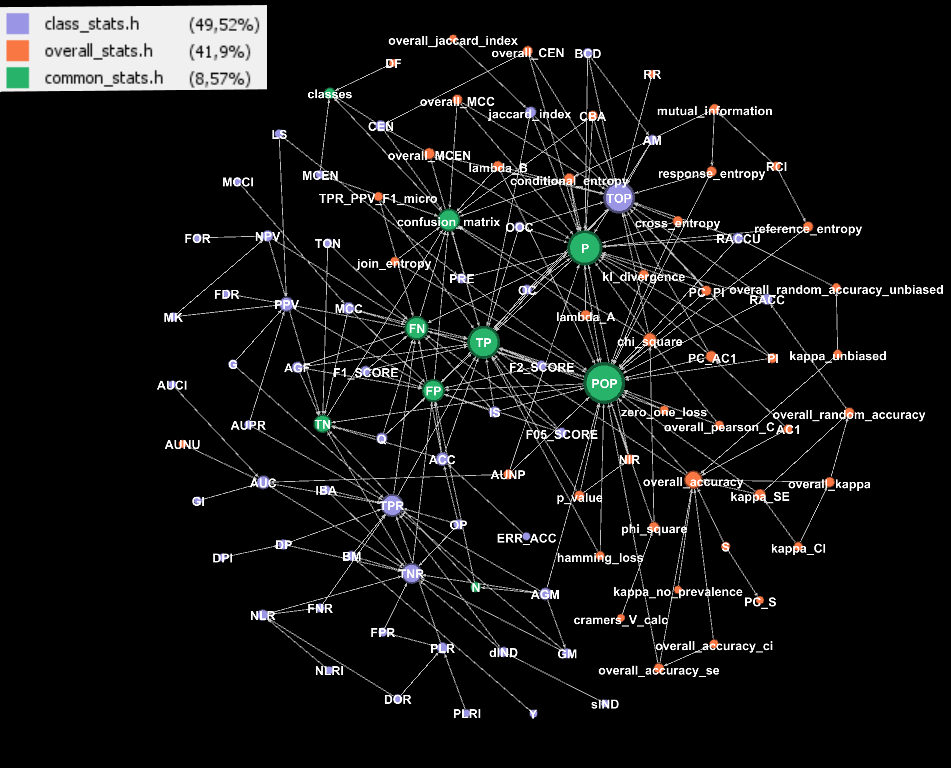
\includegraphics[width=0.6\textwidth]{scorer_net.png}
\caption{Multi class score interaction graph.
Each node identify a different performance evaluator and link are given by the interaction between the mathematical formulation of each quantity.
The graph has more than 100 nodes and more than 200 links.
The node colors are given by the classes identified in the work of Sepand et al.~\cite{PyCM}.
}
\label{fig:scorer_net}
\end{figure}
\end{center}

The evaluation of performances is a crucial task in any Machine Learning application.
Given a set of pattern and its corresponding (true) labels we can evaluate the efficiency of the understudy model with a comparison between them and the output of the model, i.e the predicted labels.
There are a lot of different scores that can be computed and any of them evaluate some aspects of the model efficiency.
Any paper author chose the score that better highlight the advantages of its model and it is difficult to move around this large zoo of indicators.
Moreover (it is quite a constant in scientific research) when a paper is send to a peer-review in many cases the reviewer suggests to the author to check if other performance indicators are good enough for the showed results.
This means that a lot of large simulations should be performed again and the appropriated variables re-computed to obtained the requested score.

At this point the main question is: are these scores totally independent one from each other?
The brief answer is simply no.
In a very interesting work of Sepand et al.~\cite{PyCM} they show how we can compute the wide part of these scores starting from the evaluation of the simple confusion matrix\footnote{
  The confusion matrix is a square matrix of shapes $(N, N)$, with $N$ the total number of classes in the current problem, whose entries are the number of rights and false classification.
  In particular, each entry of the matrix represents the instances predicted in a given class.
  If the class is the right one we call it a true positive item.
  As counterpart we will have a false positive item.
}.
Sepand et al. provide a full mathematical documentation and references about the computation of this wide range of scores starting from the evaluation of the confusion matrix.

Despite the Python code provided by Sepand et al. explain this links between the mathematical quantities they stop their analysis on the scores evaluation without any interest on the optimization of these computations.
Starting from their work we can analyze the inter-connections between these mathematical formulas and extract the dependencies between the involved variables.
In particular, a score quantity can be interpreted as a node and its connections are given by the variables needed to evaluate it.
Graphs of this type are commonly called \emph{factor graphs}.
In a mathematical formulation of \emph{factor graphs} there are different kinds of nodes (variables and factors, or equations).
The focus of our analysis is not on mathematical formalism of these kind of graphs but on the visualization of the functions interaction and on the results that we can obtain from it.

In the work of Sepand et al. the authors identify three classes of functions: common statistics, class statistics and overall stats, respectively.
In Fig.~\ref{fig:scorer_net} the interaction graph of these three classes is shown.
The figure shows deeper interactions between the three classes of functions and highlights the dependencies of the different quantities.
We can also use this kind of visualization to formulate computational considerations about the order in which compute these quantities.
Since the graph is a direct graph by definition, we can start from the root node (the node without links which bring to it) and cross the network until the leaf nodes (nodes without link which go out from the node) like in a tree-graph.
At each step of the percolation the incoming nodes identify totally independent quantities.
This independences means that the node-quantities can be potentially computed in parallel.
To clarify this considerations we can re-organize the graph visualization minimizing the link lengths and obtain a stratified graph in which each level identifies a potentially parallel section.
A graph with these properties can be obtained using the \emph{dot} visualization and it is shown in Fig.~\ref{fig:scorer_parallel}.
As can be seen in the figure we can identify 7 levels in the graph and so 7 potentially parallel regions for the computation of the full set of functions.

\begin{center}
\begin{figure}[htbp]
\hspace{-2cm}

\includegraphics[width=1.3\textwidth]{scorer_parallel.pdf}
\caption{Re-organization of the graph in Fig.~\ref{fig:scorer_net}.
The rendering was obtained using the \emph{dot} visualization, i.e the minimization of the link lengths.
The direct graph identifies the tree of dependencies and each level of the tree represents a set of independent functions that can be potentially computed in parallel.
This graph is used as parallel scheme for the \emph{Scorer} library.
}
\label{fig:scorer_parallel}
\end{figure}
\end{center}

These considerations allow the creation of the optimized version of the code of Sepand et al., the \emph{Scorer} library~\cite{Scorer}.
The \emph{Scorer} library is the C++ porting of the \emph{PyCM} library of Sepand et al. with a \emph{Cython} wrap for the Python compatibility.
Following the pre-told graph the computation of the score quantities are performed in parallel according to the levels of the tree-graph in Fig.~\ref{fig:scorer_parallel}.
The parallelization strategy chosen uses the \textsf{section} keyword of OpenMP library to perform no-wait task that are computed by each thread of the parallel region.

The graph covers more than 100 different quantities so writing the full set of parallel sections becomes an hard work in C++.
Moreover the updating of the graph with new quantities requires the updating of the full code and also of the parallelization strategy.
Each function was written as an anonymous-struct, i.e a functor, with an appropriate operator overloading.
Moreover each functor has a name given by a pre-determined regex (\textsf{get\_\{function\}}) and the list of argument follows the same nomenclature\footnote{
  If the functor receives in input the variable $A$ and $B$ we have to ensures that two functors named $get\_A$ and $get\_B$ will be provided.
  The only exception is given by the root functor.
}.
With these expedients we created a fully automated creation of the C++ script which parses the list of above functors, it computes the dependency graph and the parallelization levels and give back a compilable C++ script with the desired characteristics.
In this way we can guarantee an easy way to update the library and moreover we overcome the boring writing of a long code.
The automatic pipeline creation script is provided in the \emph{Scorer} library and can be used at each pull request or version update.

For a pretty/useful visualization of the computed quantities we render the interaction graph in an HTML framework.
In this way in each node we can insert with a CSS table the computed values that can be discovered passing the mouse over the figure.
An example of this rendering is given in the on-line version of the library~\cite{Scorer}.

In conclusion the developed \emph{Scorer} library is a very powerful tool for Machine Learning performances evaluation which can be used either in C++ either in Python codes through the \emph{Cython} wrap.
The code is automatically generated at each update and automatically tested using Continuous Integration for any platform\footnote{
  We perform tests for Unix and Windows environments.
  We check more than 15 combinations of environments and compilers.
}.
The code can be compiled using CMakefile or Makefile and a setup is provided for the Python version.
So when you write a new paper on Machine Learning and you do not know what could be the most appropriate indicator to show in your research or you are afraid that a referee could ask you to compute an other one there is only one solution: compute them all using \emph{Scorer}.


\end{document}
